\section{Background}
\label{sec:background}
% This will give all the background of the project including

% Background of the problem to be solved.
% Existing solutions/approaches to the problem, if any exist, and a comparison with the solution produced in the project.
% Reading and research done to understand existing approaches, acquire the necessary information and skills to carry out the project.
% A clear statement of the project requirements.
% References to all sources consulted are expected.

This section recalls some notions used in the project with relevant researches.
The notion of \emph{Bisimulation} is introduced as the target logic feature that needs to be learned.
The notion of \emph{Artificial Neural Networks} is introduced as the object that studied in the project.

%==================

\subsection{Bisimulation}\label{sec:bac:bis}
Bisimulation is an important concept. 
It has been introduced in many different fields and plays a very important role.
In modal logic, it was discovered when researches started to study the expressiveness for the logic, in 1970 \cite{Sangiorgi2009}.
Then that was developed by Van Benthem \cite{VanBenthem1976} who came up with \emph{p-relation} that define a symmetric directional relationship between models, i.e. bisimulation.
In computer science, the concept was introduced by Milner while studying concurrency theory \cite{Milner1990}.
The notation was developed to test the equivalence of processes in Calculus of Communication System \cite{Park1981}.
In the set Theory, it was used to determine if the equal objects can be identified with certain model \cite{Sangiorgi2009}.
Also, in formal verification, while describing a system, bisimulation was used to minimise the space of states \cite{Roscoe1994}.

Some of the past solutions for the bisimulation problem is from the perspective of the set theory.
One approach to this problem was studied by Kanellakis and Smolka while studying the equivalence testing of the calculus of communicating systems expression \cite{Milner1980}.
Originally they designed the algorithm to test the equivalence called congruence of finite state processes in CCS \cite{Paige1987}.
The algorithm was given with $O(mn)$ in time and $O(m+n)$ in space.
Another approach was given by Paige and Tarjan \cite{Paige1987}.
They converted the problem as relational coarsest partition problem.
By refining with respect to old blocks rather than current blocks, they reduce the running time into $O(m\log n)$.
Both of them did not solve the problem directly. 
By using a group of reasoning on different perspectives, they convert the problem into a clear and easier problem. 
In this project, the learning algorithm will base on the work of \cite{Paige1987}.

For the first part of the project, the baseline algorithm will use the algorithm based on the set theory. 
In the algorithm, one logical is regarded as a \emph{non-well-founded set}. 
``Such a set has an infinite descending membership sequence" i.e. the elements of the set recursively consisting itself \cite{Aczel}.
Mathematically, in this part the multi-directed graph (logic structure) $G = \langle N, E \rangle$ is regarded as a group of sets where each set represents a \emph{accessible pointed graphs}.
Edges resents membership, that is edge $\langle m, n \rangle$ (also $m \rightarrow n$) means that node $m$ has node $n$ as a element (also $n \in m$).
Then naturally, these sets will be \emph{non-well-founded sets}.
Thus extensionality axiom (two objects are equal if and only if they contain the same elements) cannot be used to define the bisimulation, since these sets may lead to cyclic arguments.
In this project, the baseline algorithm will base on the definition from \cite{Dovier2004}.
\begin{defin}
Given two graphs $G_1=\langle N_1, E_1 \rangle$ and $G_2=\langle N_2, E_2 \rangle$, a bisimulation between $G_1$ and $G_2$ is a relation $b\subseteq N_1 \times N_2$ such that
\renewcommand{\labelenumi}{\arabic{enumi})}
\begin{enumerate}
    \item $u_1b u_2 \wedge \langle u_1, v_1 \rangle \in E_1 \Rightarrow \exists v_2 \in N_2(v_1b v_2 \wedge \langle u_2, v_2 \rangle \in E_2)$
    \item $u_1b u_2 \wedge \langle u_2, v_2 \rangle \in E_2 \Rightarrow \exists v_2 \in N_2(v_1b v_2 \wedge \langle u_1, v_1 \rangle \in E_1)$
\end{enumerate}
\end{defin}
Also, for understanding purpose, a more common definition from the perspective of Kripke model \cite{Glabbeek2011} is given.
Here the multi-directed graph (logic structure) are labelled transition system (LTS), denoted as $(S, \rightarrow, \models)$ with the set of actions $A$ and the set of predicates $P$. $S$ stands for a class of states, $\rightarrow$ stands for a collection of binary relations $\stackrel{a}{\rightarrow}\subseteq S\times S$ where $a \in A$. 
And $\models \subseteq S \times P$, where $s\models p$ indicate that predicate $p \in P$ holds in state $s \in S$ \cite{Glabbeek2011}. Definition in this prospect is given below \cite{Glabbeek2011}.
\begin{defin}
Let $(S, \rightarrow, \models)$ be an LTS over $A$ and $P$. A bisimulation is a binary relation $R \subseteq S \times S$, satisfying:
\renewcommand{\labelenumi}{\arabic{enumi})}
\begin{enumerate}
    \item if $sRt$, then $s \models p \leftrightarrow t \models p$ for all $p\in P$.
    \item if $sRt$ and $s \stackrel{a}{\rightarrow}s'$ with $a \in A$, then there exists a $t'$ with $t \stackrel{a}{\rightarrow} t'$ and $s'Rt'$
    \item if $sRt$ and $t \stackrel{a}{\rightarrow} t'$ with $a\in A$, then there exists an $s'$ with $s \stackrel{a}{\rightarrow}s'$ and $s'Rt'$
\end{enumerate}
\end{defin}

%======================

\subsection{Artificial Neural Networks (ANNs)}
For the second part of the project, the capability of the MLPs for catching the bisimulation equivalence is explored. 
Here MLPs is chosen as the representative of ANNs as a kind for machine learning methods.
Generally, machine learning can be defined as an experience-base computational method \cite{Mohri2013}.
Mohri pointed out that machine learning is mainly used in the classification, regression, ranking, clustering and dimensionality reduction \cite{Mohri2013}.
Among all the machine learning methods ANN is a unique architecture which is good at the pattern related problems \cite{Dayhoff1990}.
This architecture is inspired by the neural cell in the brain. 
By simulate neural cell, a neural network is prospected to learn from experience also understand the logic concepts. 
In 1943, McCulloch and Pitts carried out the first neural network, namely the McCulloch-Pitts Neuron \cite{Dayhoff1990}. 
It is a binary discrete-time element with excitatory, that comes to the perception which can learn the patterns through supervised learning.
And for multilayer perceptron (MLP), it is a feed forward artificial neural network.
A MLP has an input layer, an output layer and at least one hidden layer \cite{rosenblatt1961principles} (See Fiture \ref{fig:mlp}).
More importantly, most ANNs are developed base on the MLP.

\begin{figure}[h]
    \centering
    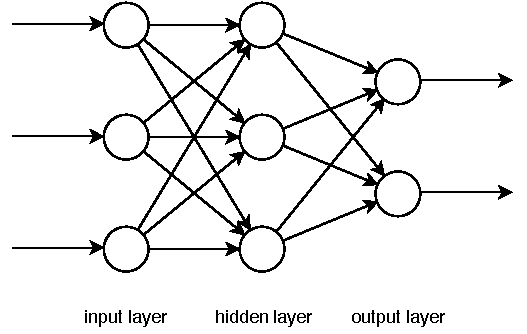
\includegraphics[width=0.5\textwidth]{img/eg_mlp.pdf}
    \caption{Typical MLP}
    \label{fig:mlp}
\end{figure}

While research on logic and ANN has been studied. 
Logic or symbolic system is more expressive and more readable for human. 
Learning base on a symbolic system has less dependence on data.
While commonly, the neural network is known as a less formal system short at human reasoning.
Thus, neuro-symbolic integration is growing rapidly.
It has been shown that feedforward connectionist networks are able to compute certain semantics operators in positional logic programs and approximate them in first-order logic \cite{HITZLER2004245}.
Also, there are scholars constructed recurrent connectionist networks that can approximate logic program and its semantics \cite{holldobler1999approximating, Holldobler91towardsa}.
Further, for the logic relation, a system PAN who accept symbolic input as the condition of the logical rule is developed \cite{guillame2010first}.
There are also research investigates the neural network approach for the first-order abductive inference\cite{Ray_aneural}.

However, this project will focus on MLP and bisimulation only.
Because MLP is the most typical neural network and is part of many neural networks.
By study, the capability, the compute ability of MLPs with certain depth will be evaluated.

% TODO: activation function 

% \subsection{Library Used}
% TODO
% \subsection{Cloud Computing}
% TODO